\hypertarget{capacity-to-distinguish-pirhotext-colbisbm-from-iidtext-colbisbm-and-other-variants}{%
\section{\texorpdfstring{Capacity to distinguish
\(\pi\rho\text{-}colBiSBM\) from \(iid\text{-}colBiSBM\) and other
variants}{Capacity to distinguish \textbackslash pi\textbackslash rho\textbackslash text\{-\}colBiSBM from iid\textbackslash text\{-\}colBiSBM and other variants}}\label{capacity-to-distinguish-pirhotext-colbisbm-from-iidtext-colbisbm-and-other-variants}}

The idea of this model selection simulations is to assess how the model
select the correct \emph{colBiSBM} model among the possible ones:
\textit{iid, pi, rho, pirho}. This difference being based on the row and
col block proportions.

For this task we choose the same simulation context as
\cite{chabert-liddellLearningCommonStructures2023}.

Namely \(n_{1}^{m} = 90, n_{2}^{m} = 90, Q_1 = Q_2 = 3\),
\(\bm{\alpha}, \bm{\pi}\) and \(\bm{\rho}\) are set as follows:

\begin{align*}
    \bm{\alpha} =.25 +  \begin{pmatrix}
                        3 \eps[\alpha] & 2 \eps[\alpha] & \eps[\alpha] \\
                        2 \eps[\alpha] & 2 \eps[\alpha] & - \eps[\alpha] \\
                        \eps[\alpha] & - \eps[\alpha] & \eps[\alpha]
                    \end{pmatrix}, & & \bm{\pi}^1 = \begin{pmatrix}
                        \frac{1}{3}, & \frac{1}{3}, & \frac{1}{3}
                    \end{pmatrix}, & & \bm{\pi}^2 = \sigma\begin{pmatrix}
                        \frac{1}{3} - \eps[\pi], & \frac{1}{3}, & \frac{1}{3} + \eps[\pi]
                    \end{pmatrix},\\
    & & \bm{\rho}^1 = \begin{pmatrix}
                        \frac{1}{3}, & \frac{1}{3}, & \frac{1}{3}
                    \end{pmatrix}, & & \bm{\rho}^2 = \sigma\begin{pmatrix}
                        \frac{1}{3} - \eps[\rho], & \frac{1}{3}, & \frac{1}{3} + \eps[\rho]
                    \end{pmatrix},
\end{align*} with \(\eps[\alpha] = 0.16\), \(\eps[\pi]\) and
\(\eps[\rho]\) taking 9 values equally spaced in
\(\left[ 0, .28\right]\). We simulate 324 different collections for each
value of \(\eps[\pi]\) and \(\eps[\rho]\).

\(\pi\rho\text{-}colBiSBM\), \(\pi\text{-}colBiSBM\),
\(\rho\text{-}colBiSBM\), \(iid\text{-}colBiSBM\) and
\(sep\text{-}colBiSBM\) are put in competition and the model with the
greater BIC-L is selected as the \emph{preferred model}.

When \(\eps[\pi] = 0\), \(\bm{\pi}^1 = \bm{\pi}^2\), \(\eps[\rho] = 0\)
and \(\bm{\rho}^1 = \bm{\rho}^2\), the generated collection is an
\(iid\text{-}colBiSBM\). When \(\eps[\pi] > 0\) or
\(\bm{\pi}^1 \neq \bm{\pi}^2\), the model is a \(\pi\text{-}colBiSBM\).
When \(\eps[\rho] > 0\) or \(\bm{\rho}^1 \neq \bm{\rho}^2\), the model
is a \(\rho\text{-}colBiSBM\). Finally, when \(\eps[\pi] > 0\) or
\(\bm{\pi}^1 \neq \bm{\pi}^2\) and \(\eps[\rho] > 0\) or
\(\bm{\rho}^1 \neq \bm{\rho}^2\), the model is a
\(\pi\rho\text{-}colBiSBM\).

\begin{table}[!h]

\caption{\label{tab:tables}\label{tab:pi-model-sel}Model selection for varying $\pi$ mixture parameters}
\centering
\begin{tabular}[t]{lccccl}
\toprule
\multicolumn{1}{c}{ } & \multicolumn{4}{c}{Proportions of model selection} & \multicolumn{1}{c}{Blocks} \\
\cmidrule(l{3pt}r{3pt}){2-5} \cmidrule(l{3pt}r{3pt}){6-6}
$\eps[\pi]$ & $iid\text{-}colBiSBM$     & $\pi\text{-}colBiSBM$ & $\rho\text{-}colBiSBM$ & $\pi\rho\text{-}colBiSBM$ & Recovered $Q_1$\\
\midrule
0.00 & 0.65 & 0.00 & 0.35 & 0.00 & 3.00\\
0.04 & 0.66 & 0.00 & 0.34 & 0.00 & 3.00\\
0.07 & 0.64 & 0.01 & 0.34 & 0.01 & 3.01\\
0.11 & 0.63 & 0.03 & 0.31 & 0.03 & 3.01\\
0.14 & 0.55 & 0.12 & 0.28 & 0.05 & 3.00\\
\addlinespace
0.18 & 0.39 & 0.26 & 0.21 & 0.13 & 3.01\\
0.21 & 0.23 & 0.42 & 0.13 & 0.23 & 3.01\\
0.25 & 0.10 & 0.56 & 0.05 & 0.29 & 3.02\\
0.28 & 0.01 & 0.65 & 0.01 & 0.33 & 3.01\\
\bottomrule
\end{tabular}
\end{table}

\begin{table}[!h]

\caption{\label{tab:tables}\label{tab:rho-model-sel}Model selection for varying $\rho$ mixture parameters}
\centering
\begin{tabular}[t]{lccccl}
\toprule
\multicolumn{1}{c}{ } & \multicolumn{4}{c}{Proportions of model selection} & \multicolumn{1}{c}{Blocks} \\
\cmidrule(l{3pt}r{3pt}){2-5} \cmidrule(l{3pt}r{3pt}){6-6}
$\eps[\rho]$ & $iid\text{-}colBiSBM$     & $\pi\text{-}colBiSBM$ & $\rho\text{-}colBiSBM$ & $\pi\rho\text{-}colBiSBM$ & Recovered $Q_2$\\
\midrule
0.00 & 0.63 & 0.37 & 0.00 & 0.00 & 3.00\\
0.04 & 0.65 & 0.34 & 0.00 & 0.01 & 3.00\\
0.07 & 0.64 & 0.33 & 0.01 & 0.01 & 3.00\\
0.11 & 0.64 & 0.31 & 0.03 & 0.02 & 3.00\\
0.14 & 0.53 & 0.29 & 0.11 & 0.06 & 3.00\\
\addlinespace
0.18 & 0.42 & 0.20 & 0.24 & 0.14 & 3.01\\
0.21 & 0.25 & 0.12 & 0.40 & 0.22 & 3.01\\
0.25 & 0.08 & 0.06 & 0.58 & 0.29 & 3.01\\
0.28 & 0.01 & 0.01 & 0.65 & 0.32 & 3.00\\
\bottomrule
\end{tabular}
\end{table}

\begin{figure}[H]
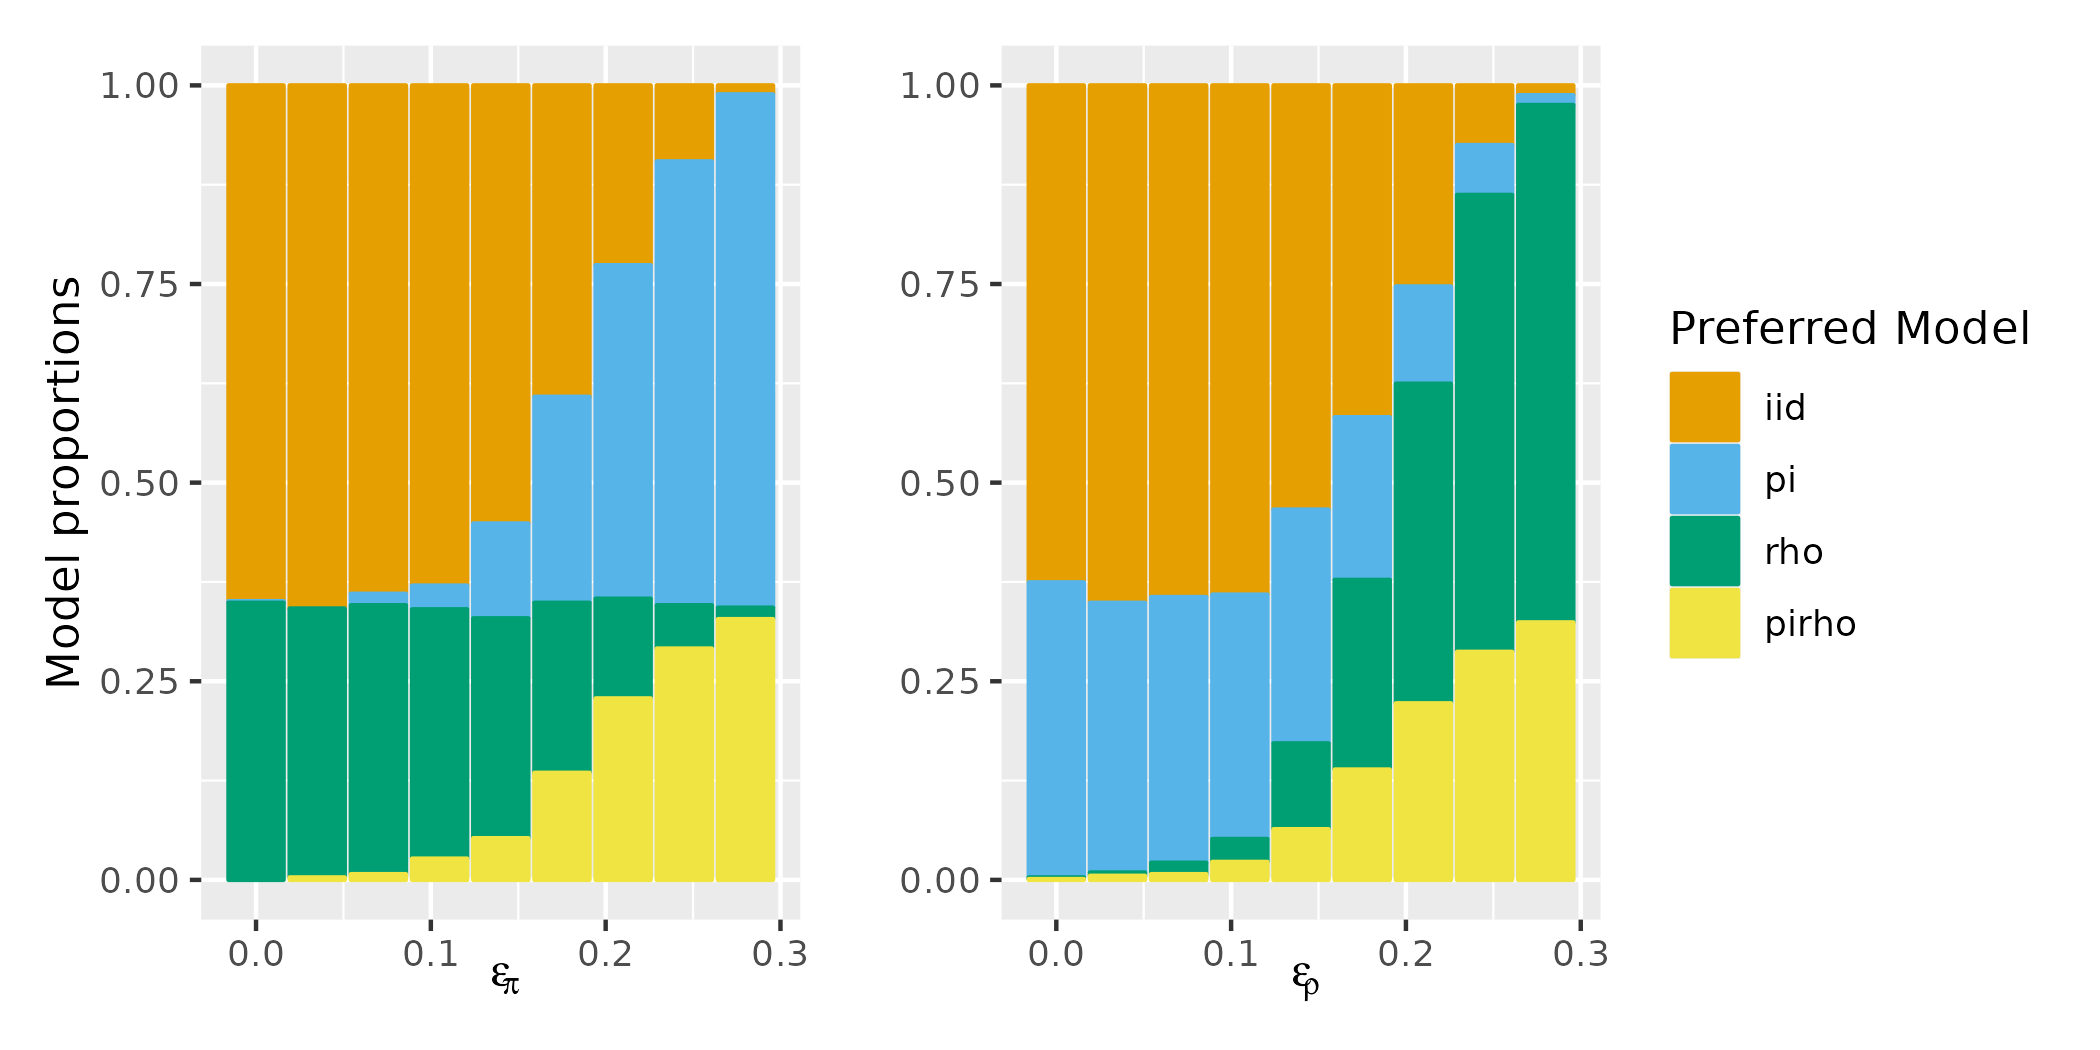
\includegraphics{./Rcodes/simulation/img/plot_model_function_eps.png}
\caption{Plot of preferred model in function of $\eps[\pi]$ and $\eps[\rho]$}
\label{fig:pref_model_func_eps}
\end{figure}

\paragraph{Results:}

On the figure \ref{fig:pref_model_func_eps} and tables
\ref{tab:pi-model-sel} and \ref{tab:rho-model-sel}, one can see that
there is a turning point around \(\eps[\pi] = 0.2\) (resp.
\(\eps[\rho] = 0.2\)), before which \(iid\text{-}colBiSBM\) and
\(\rho\text{-}colBiSBM\) (resp. \(\pi\text{-}colBiSBM\)) are selected
most of the times and after \(0.2\) the \(\pi\text{-}colBiSBM\) (resp.
\(\rho\text{-}colBiSBM\)) and \(\pi\rho\text{-}colBiSBM\) gets more and
more selected, highlighting our capacity to recover the simulated
structure.

\paragraph*{Remark:}

Please note that when ``Recovered \(Q_1\)(or \(Q_2\))'' is not an
integer it's because some procedures returned a value other than 3.
